\section{AnImaX Projekt}
Die Entwicklung des AnImax-Projekts entspringt als ein Teil des FlexIX-Projekts des Bundesministerium für Bildung und Forschung. Das Kooperationsprojekt zwischen der TU Berlin und der Hochschule Koblenz wurde ursprünglich als Messstation für die P04 Beamline bei Petra III (DESY Hamburg) entworfen, kann jedoch auch an anderen Synchrotrons (z.B. BESSY II, HZB Berlin) mit einer Energiespanne von \SI{200}{\electronvolt}-\SI{3000}{\electronvolt} genutzt werden. Es handelt sich um einen experimentellen Aufbau mit STXM im full-field-Modus oder STXM mit optionaler Detektion des Fluoreszenzsignals.
\subsection{Experimenteller Aufbau}
Der optische Aufbau (\cref{fig:animaxsetup}) befindet sich in einer Messkammer im Hochvakuum bei etwa \SI{e-6}{\milli\bar}. Davor ist eine weitere Messkammer im Hochvakuum (\SI{5e-7}{\milli\bar}) direkt an die Beamline angeschlossen. Sie dient als differentielle Pumpstrecke für das Ultrahochvakuum der Beamline (\SI{e-9}{\milli\bar}). Aus dem von der Beamline kommenden Synchrotronstrahl wird eine Wellenlänge selektiert. Der Strahl trifft auf eine Fresnelsche Zonenplatte mit einer Brennweite von \SI{7}{\milli\meter} (bei \SI{700}{\electronvolt}). Die äußere Zonenweite ist \SI{45}{\nano\meter}, der Außendurchmesser beträgt \SI{333}{\micro\meter}. Die Mittenstop hat einen Durchmesser von \SI{160}{\micro\meter} und filtert gemeinsam mit der OSA (OSA = \textit{order sorting aperture}) zusammen alles bis auf die 1. Ordnung des von der Zonenplatte gebeugten Lichts aus. Die OSA ist ein Pinhole mit \SI{150}{\micro\meter} Durchmesser und befindet sich mit der Zonenplatte auf einem gemeinsamen Frame, über Piezekristalle lässt sich der Abstand zwischen beiden jedoch justieren. Außerdem ist sie an einem Röhrchen fixiert, welches sich in die zentrale Öffnung des QUAD-Detektors bewegen lässt. Der Synchrotronstrahl wird also an der Zonenplatte fokussiert und passiert die OSA und das zentrierte Loch des Detektors bevor er auf die Probe trifft. Daraufhin wird ein Teil der Strahlung in Fluoreszenz umgewandelt und vom SDD registriert. Die durch die Probe transmittierte Intensität kann durch eine schnellauslesende CCD außerhalb der Messkammer detektiert werden. Da CCDs für Röntgenstrahlung die benötigten Zählraten nicht leisten können, wurde auf eine CCD, welche sensitiv für sichtbares Licht ist, zurückgegriffen. Daher ist hinter der Probe noch ein Phosphorschirm angebracht, welcher sichtbares Licht (grün) emittiert. Dieses wird durch eine Linse gesammelt und über ein Bleifenster aus der Vakuumkammer ausgekoppelt, dann durch die CCD detektiert.

\begin{figure}[H] %h:Grafik an dieser Stelle einbinden. Falls das nicht geht: %t:oben auf der Seite. Wenn dies auch nicht möglich ist: %b:am Fuß der Seite oder %p:auf der nächsten Seite %! is specified, then ignore the restrictions of placing floating objects %H (float package) forces position
  \centering
     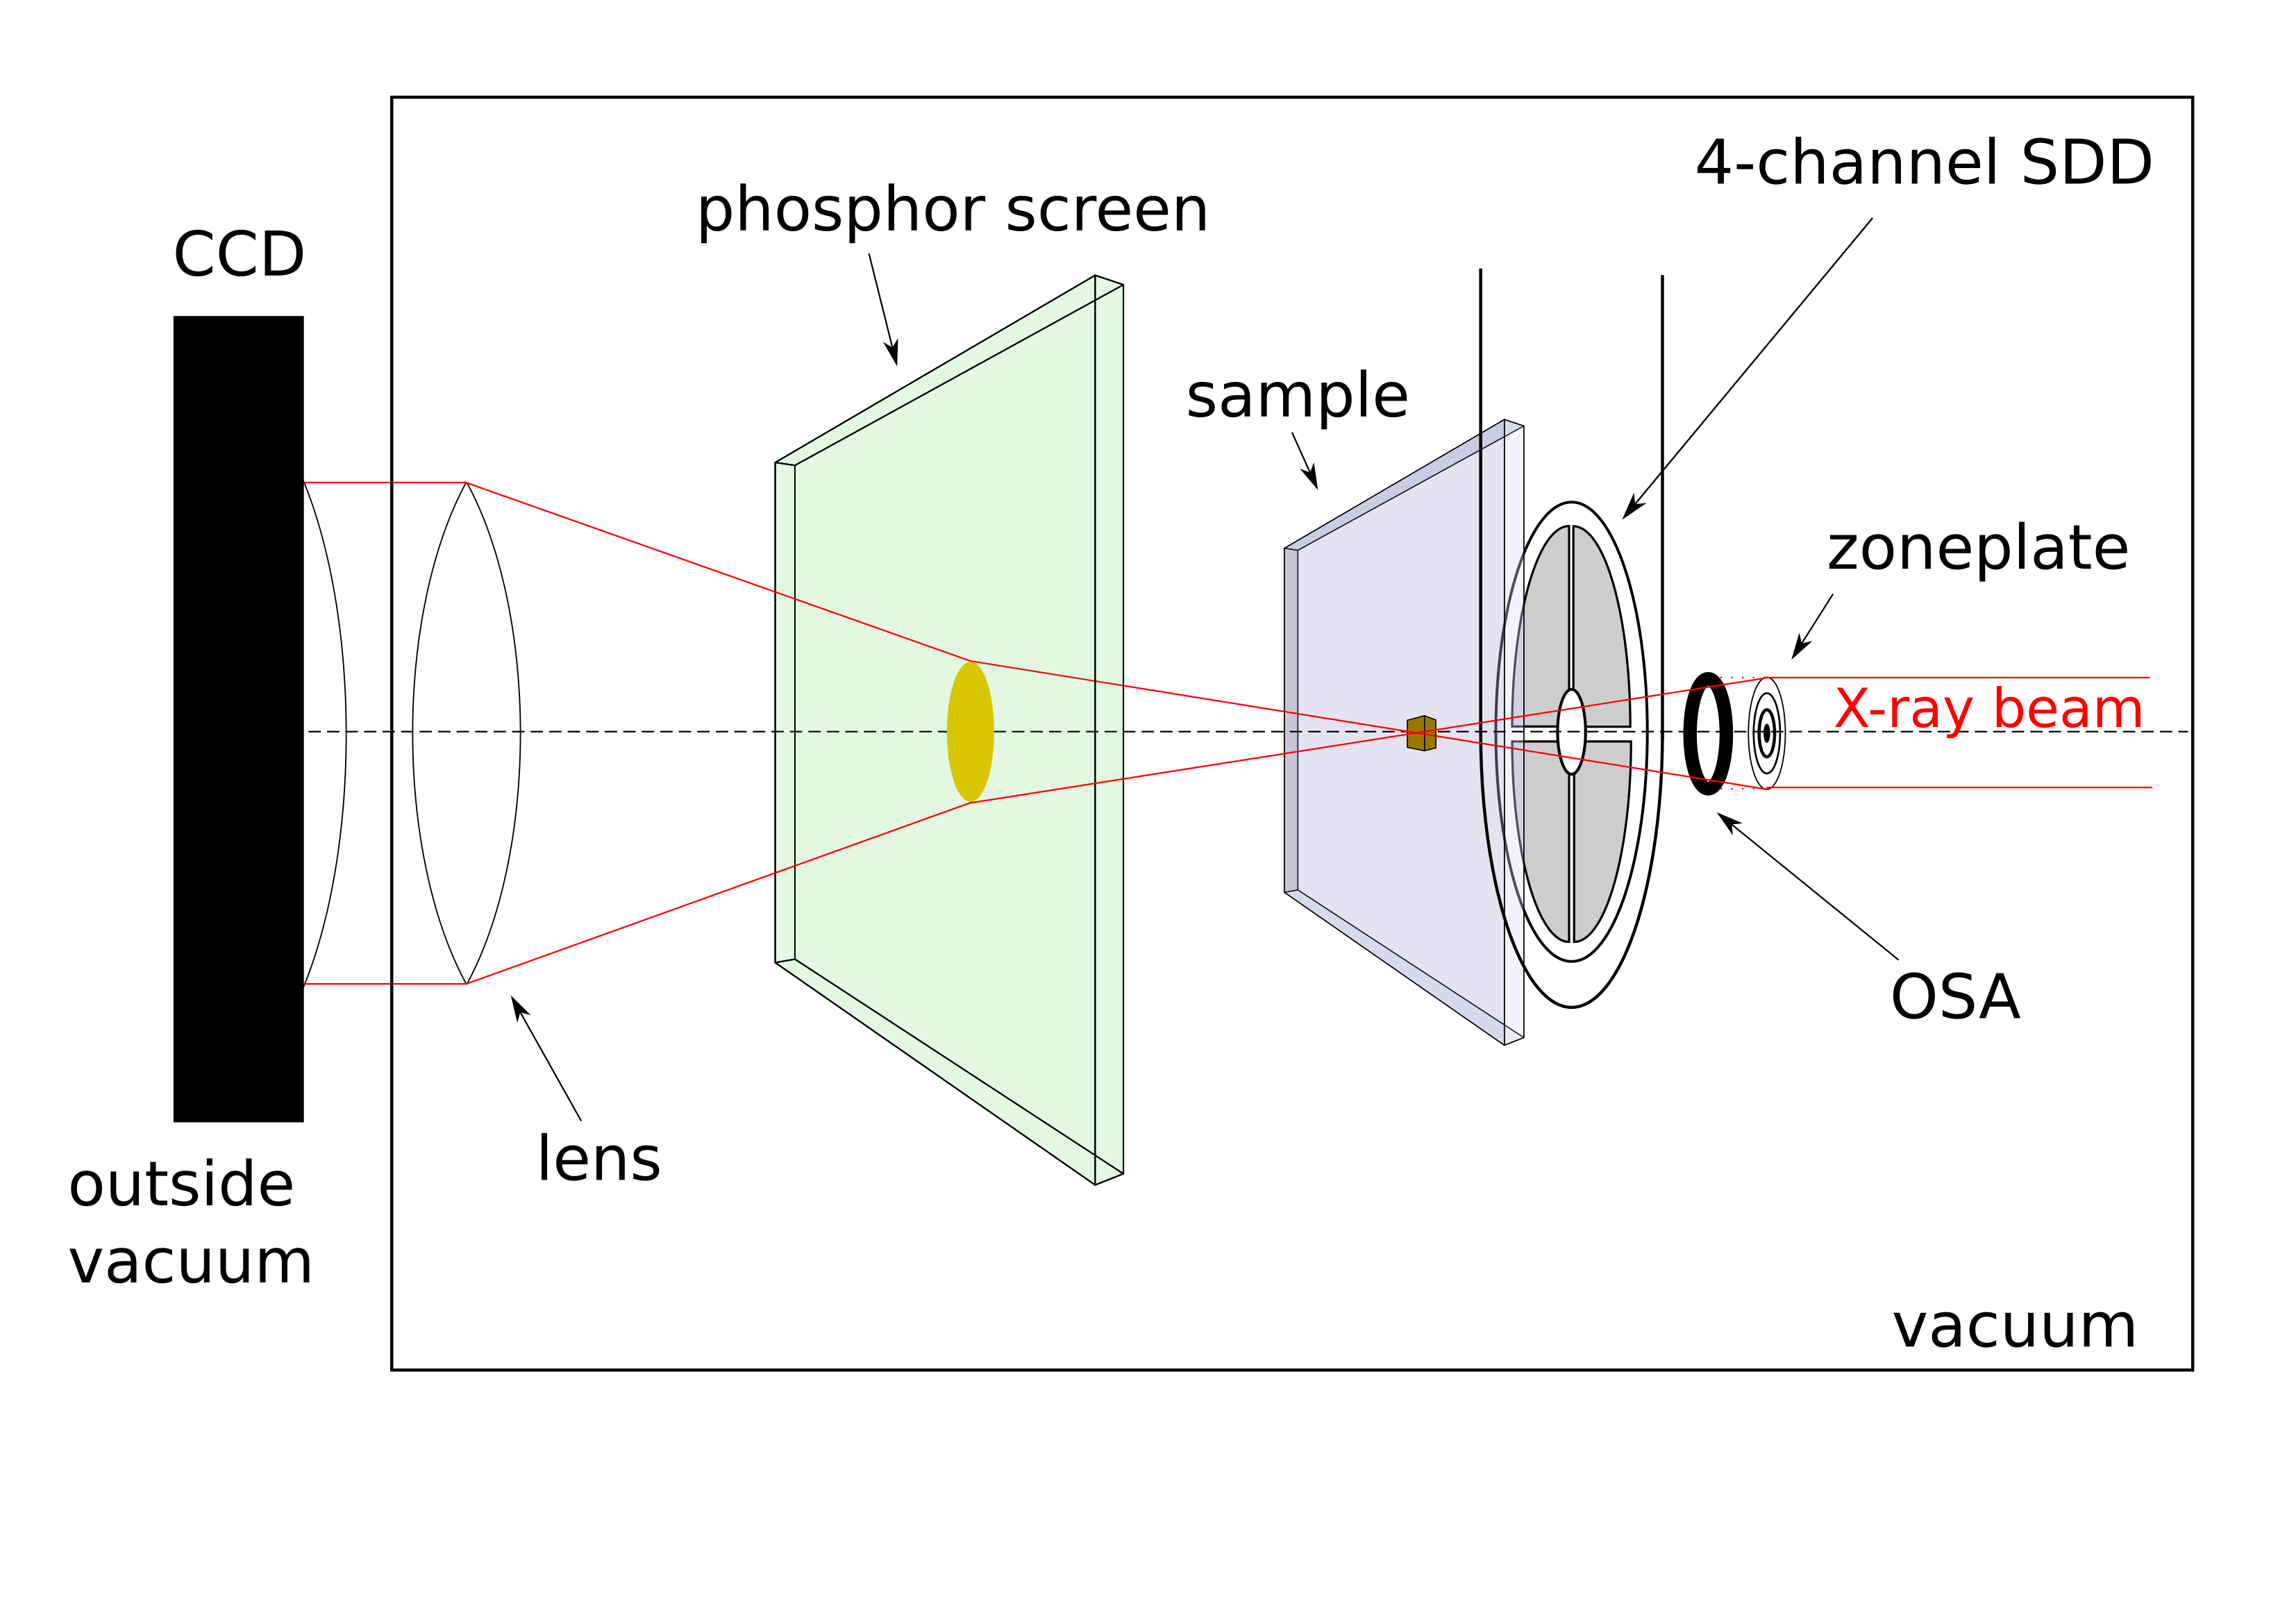
\includegraphics[width=0.9\textwidth]{illustrations/animax-gruppe_hanna.png}
  \caption[Skizze optischer Aufbau]{Der optische Aufbau im AnImaX-Projekt. Die von der Synchrotronquelle eintreffene Strahlung wird zunächst an der Zonenplatte fokussiert, höhere Ordnungen werden an der OSA aussortiert. Der Strahl passiert den QUAD-Detektor zentral und trifft auf die Probe, welche zur Fluoreszenz angeregt wird. Hinter der Probe wandelt ein Phosphorschirm das transmittierte Licht in eine für die CCD sichtbare Wellenlänge um. Das Licht wird mit Hilfe einer Linse parallelisiert und von der CCD detektiert wird \cite[S.~40]{hanna}.}
  \label{fig:animaxsetup}
\end{figure}
Über Piezokristalle lässt sich der Probenhalter bewegen. An diesem befindet sich Platz für 5 Proben, sodass ein Probentausch ohne Brechen des Vakuums möglich ist. Die Piezokristalle lassen sich x- und y-Richtung enkodiert mit einer Genauigkeit von etwa \SI{0.1}{\nano\meter} und einer Reichweite von \SI{100}{\micro\meter} fahren. Dies ermöglicht eine hohe Auflösung bei großer abgerasterter Fläche. Der Scanner Frame und damit auch die Probe können mit Hilfe einer Computersoftware gesteuert werden. Dazu sind die Piezokristalle an einen Controller und dieser an einen PC angeschlossen. Zwei Scan-Modi stehen zur Datenakquise zur Verfügung: der step-by-step-Modus und der on-the-fly-Modus, welcher kontinuierlich Daten akquiriert. Letzterer ermöglicht deutlich verkürzte Messzeiten, eine Messung mit 10000px je \SI{200}{\milli\second} Aufnahmezeit benötigt beispielsweise nur etwa eine halbe Stunde.\newlines
